\newpage
\chapter{Network Training}
\label{chapter07}

Training in classical multilayer artificial neural networks is related to optimizing the weights that characterize the connections between individual neurons. The learning task is a numerical optimization in a multidimensional space of real numbers. Many exact numerical methods and many heuristic methods have been developed in the last few decades. In the present work, the emphasis falls on two methods (one exact numerical and the other heuristic). As an exact numerical method, the Encog software library offers the widely used error backpropagation method (as well as some modifications thereof). From the group of heuristic methods, genetic algorithms with mutation modification are used according to the method of evolution of differences. The Genetic Algorithms - Apache Commons software library implements the genetic algorithm.

\section{Backpropagation of the error}

In error back propagation, in operational mode, signals travel from the input of the network to its output. The training examples are applied randomly so that the network does not learn the feed pattern but develops its generalization abilities. The total error is calculated at the network's output and then fed back, from output to input, to estimate the error each neuron contributes. After determining the individual error for each neuron, a numerical correction (according to the gradient) is performed on the weights that connect the neurons. This back-calculation gives the method its name and places it in the group of exact numerical methods that rely on the gradient to correct the weights. Essential to error backpropagation learning is that the neuron's activation function must be differentiable. The Encog library provides a group of methods for optimizing network weights.

\begin{figure}[h]
\centering
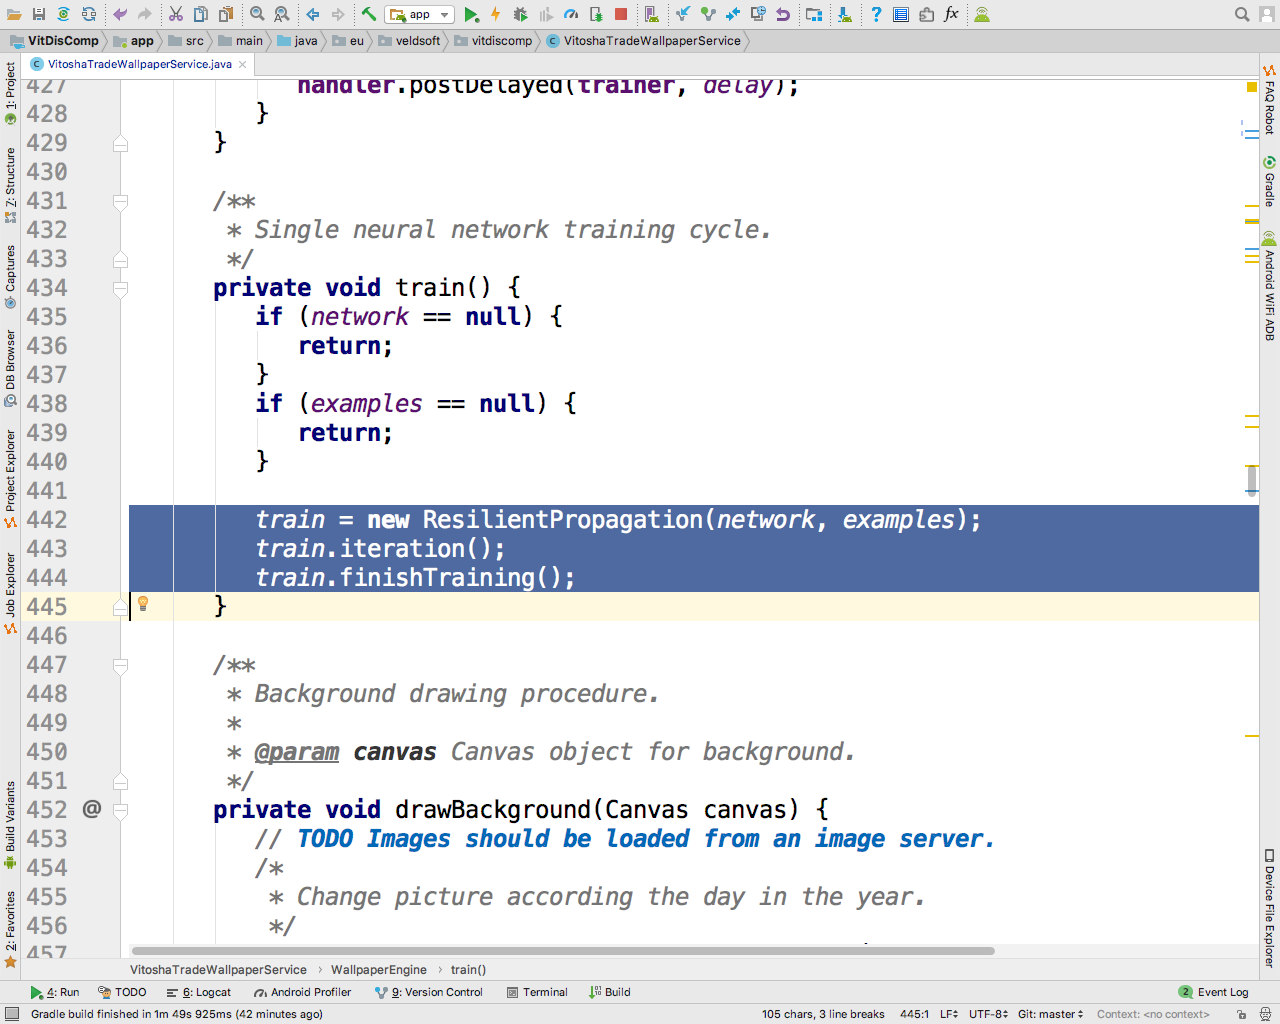
\includegraphics[height=0.45\pdfpageheight]{pic0173}
\caption{A single step to train the network}
\label{fig:pic0173}
\end{figure}
\FloatBarrier

The Encog library allows several training options with exact numerical methods, and the Resilient Propagation method, which is elastic backpropagation of the error (Fig. \ref{fig:pic0173}), is chosen in this tutorial. Elastic error propagation is a modification of the primary method in which the learning rate is determined dynamically and is not just one value for the entire network. In the classic error backpropagation approach, the learning rate is just one value, usually empirically tuned between 0.0 and 1.0. The most commonly used is 0.35, a trade-off between learning speed and reaching an optimal value for the weights (the fine-tuning of the weights in the final training phase).

\begin{figure}[h]
\centering
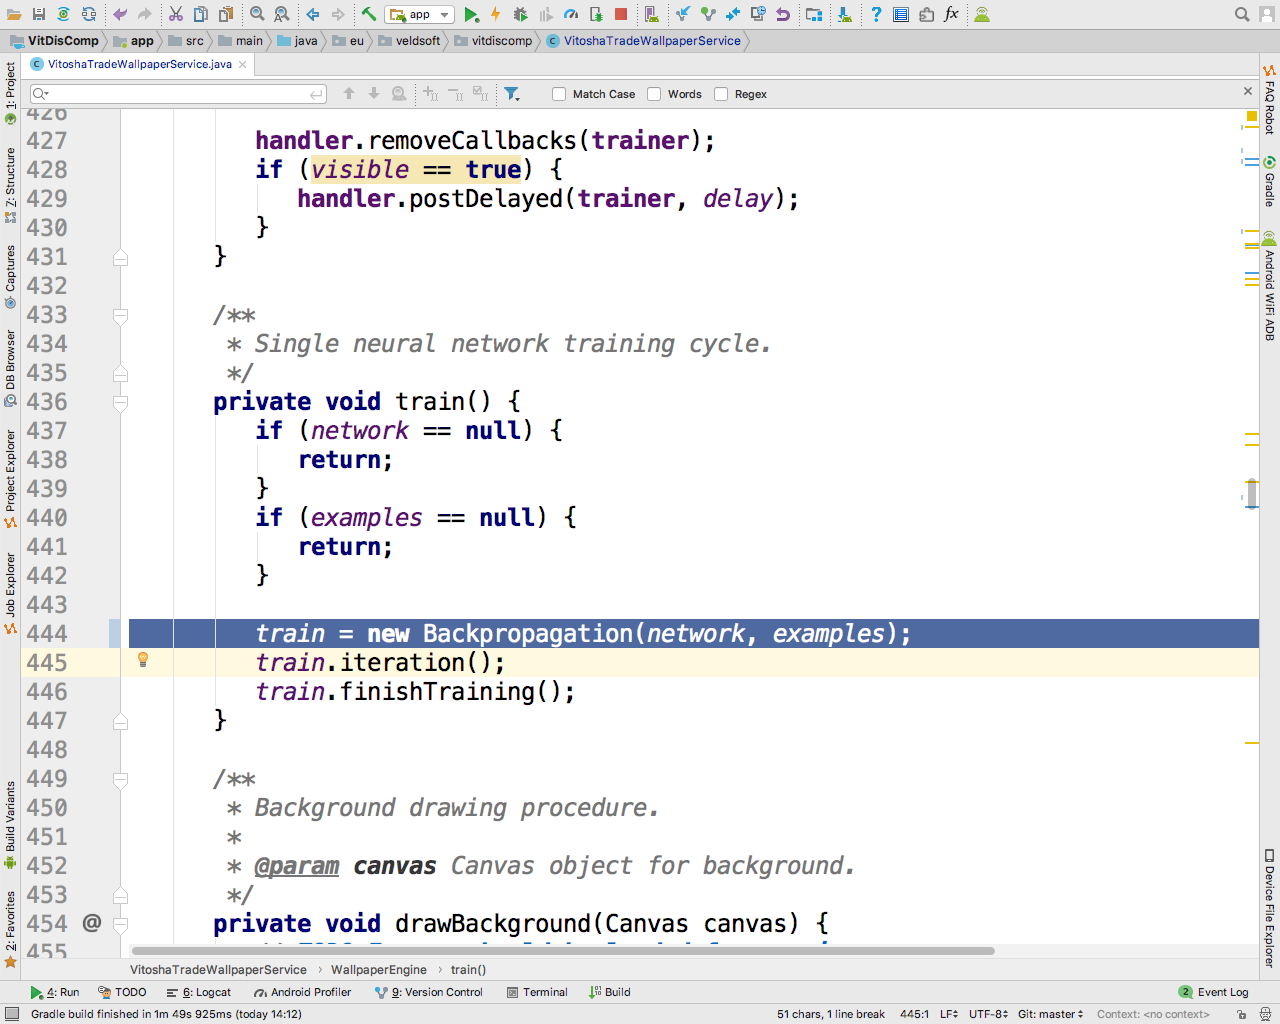
\includegraphics[height=0.45\pdfpageheight]{pic0174}
\caption{Classical backpropagation of the error}
\label{fig:pic0174}
\end{figure}
\FloatBarrier

The fact that the Encog library is written according to the canons of object-oriented programming allows us to switch to classical error backpropagation by replacing only one line (Fig. \ref{fig:pic0174}) from elastic learning.

\begin{figure}[h]
\centering
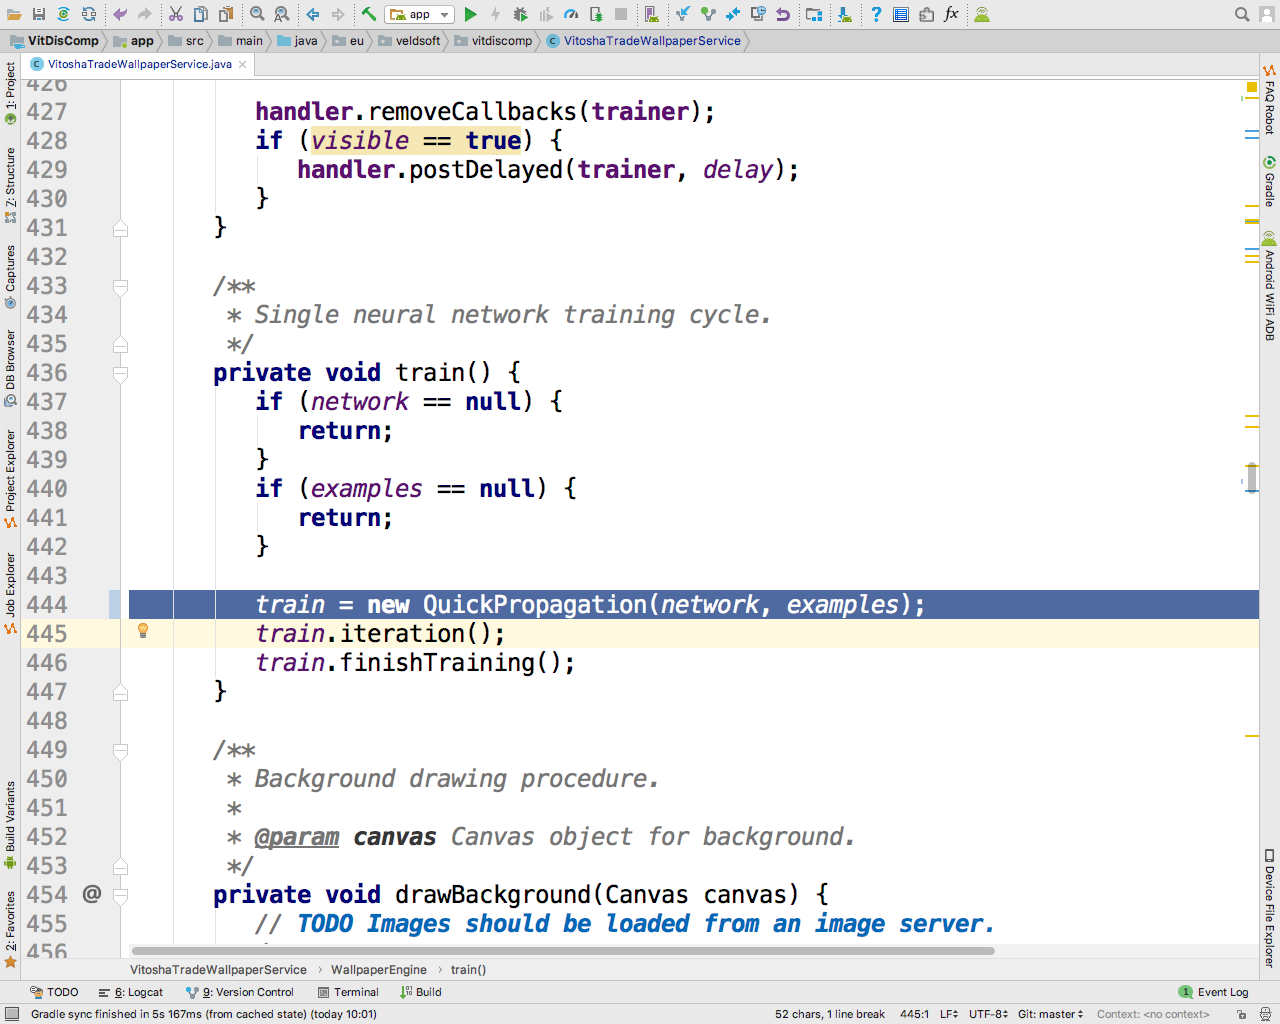
\includegraphics[height=0.45\pdfpageheight]{pic0175}
\caption{Rapid propagation of error}
\label{fig:pic0175}
\end{figure}
\FloatBarrier

With precisely the same ease, the library allows one to switch to fast error propagation (Fig. \ref{fig:pic0175}). This modification of the error backpropagation algorithm introduces an improvement by using the Newton-Rawson method to determine the second derivative further so that the additional information from the second derivative improves the way the network weights are adjusted. Thanks to this modification, more giant steps are taken along the slopes of the error function, and when approaching the extreme point, the step is reduced.

\begin{figure}[h]
\centering
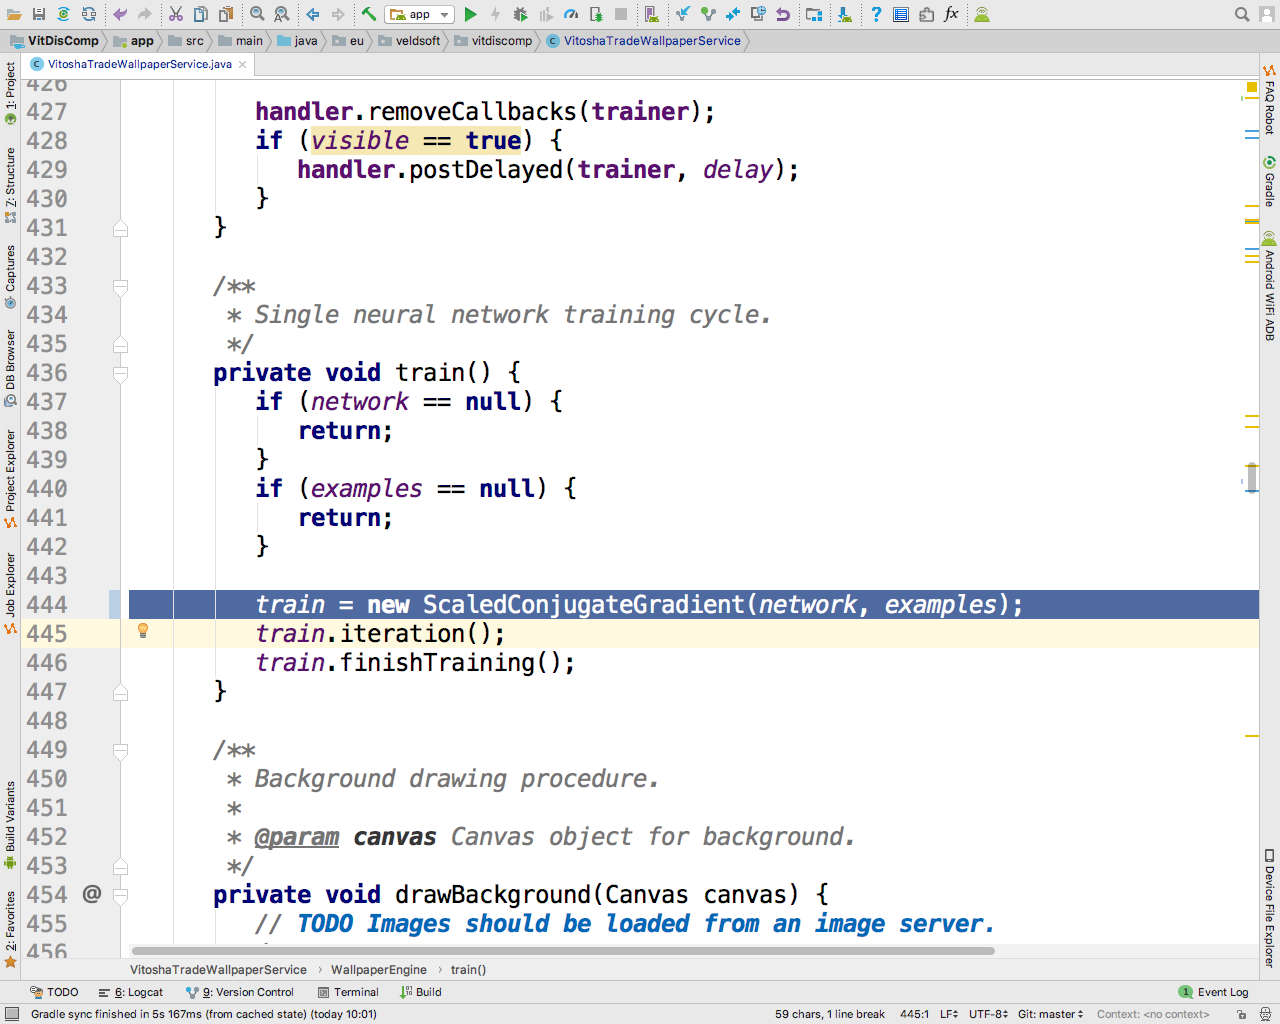
\includegraphics[height=0.45\pdfpageheight]{pic0176}
\caption{Scale gradient compound}
\label{fig:pic0176}
\end{figure}
\FloatBarrier

The scaled gradient fit (Fig. \ref{fig:pic0176}) also uses the information from the second derivative. Thus, a better path to the optimal point is found than methods that only use the first derivative. The need to use more computing resources is the price of such an improvement. The difference with this method is that the weight corrections are not always in the direction indicated by the first derivative.

\begin{figure}[h]
\centering
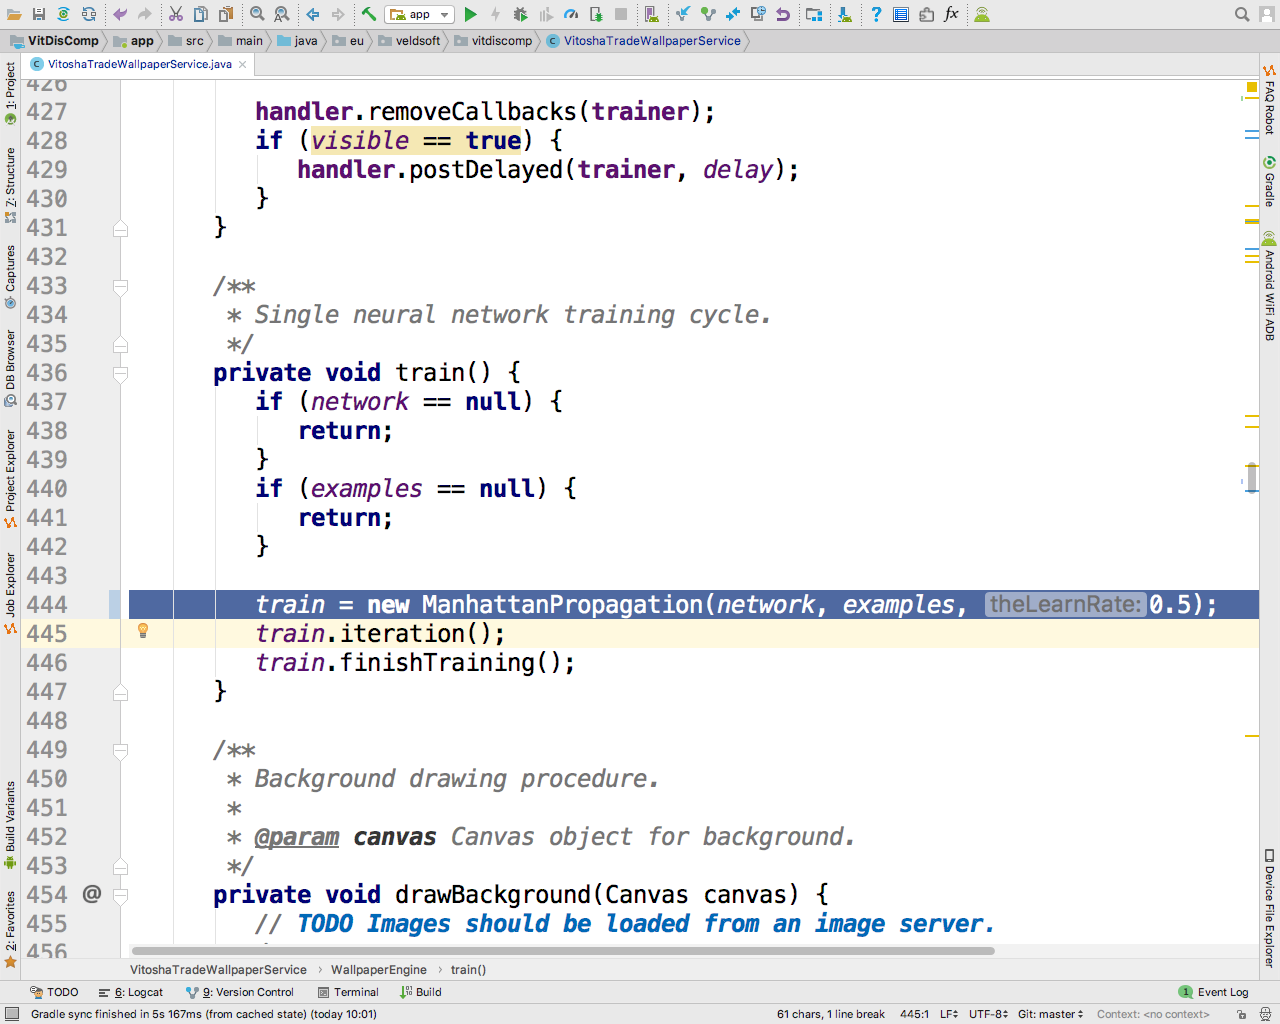
\includegraphics[height=0.45\pdfpageheight]{pic0177}
\caption{Manhattan rule weight correction}
\label{fig:pic0177}
\end{figure}
\FloatBarrier

A simplified variant of elastic learning is the adjustment of weights according to the Manhattan rule (Fig. \ref{fig:pic0177}). In this modification of the error's backpropagation, only the first derivative's direction is used, and a single, predefined value (theLearningRate) is applied to correct the weights. The benefit of this method comes from the fact that sometimes the first derivative is calculated to a value that is too large or too small. When the correction is a fixed value, and only the direction of the derivative is used, the negative effect of large/small correction values is avoided. A disadvantage of this algorithm is that the single correction value must be adaptively tuned. It is usually started with a more significant value and reduced, analogous to the simulated annealing method.

\section{Genetic Algorithms}

Although the Encog library has capabilities for training artificial neural networks with genetic algorithms (the MLMethodGeneticAlgorithm class), the Genetic Algorithms - Apache Commons library is preferred in this tutorial because it gives much more freedom to implement genetic algorithm operations and extensions towards the differential evolution method.

\begin{figure}[h]
\centering
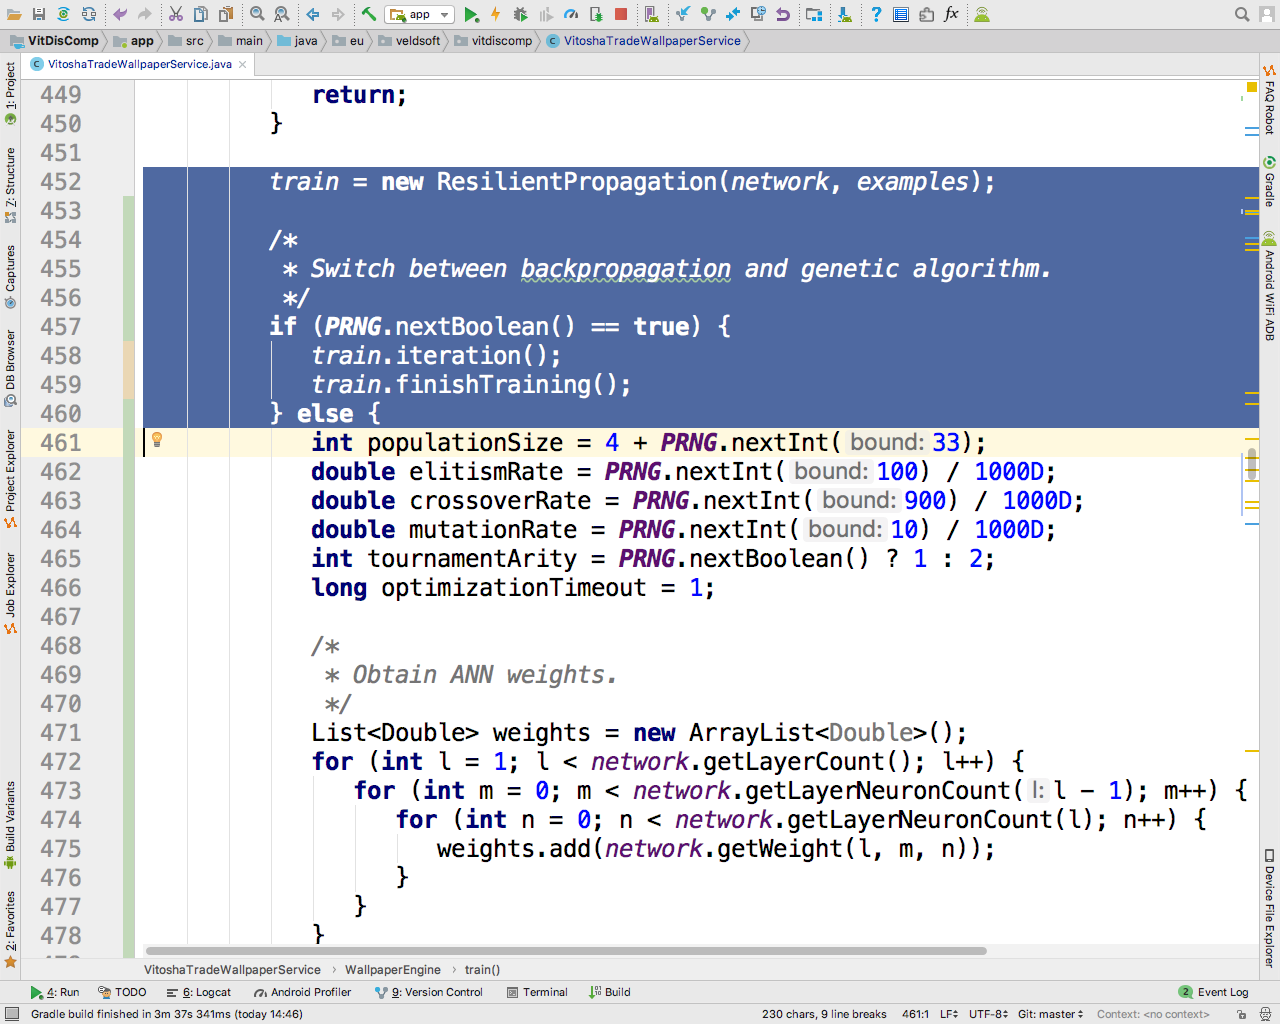
\includegraphics[height=0.45\pdfpageheight]{pic0178}
\caption{Switch between error backpropagation and genetic algorithm}
\label{fig:pic0178}
\end{figure}
\FloatBarrier

With the addition of a genetic algorithm, a hybrid system for training artificial neural networks is obtained (Fig. \ref{fig:pic0178}). Half of the cases are randomly trained with an exact numerical method, and the other half with a heuristic method.

\begin{figure}[h]
\centering
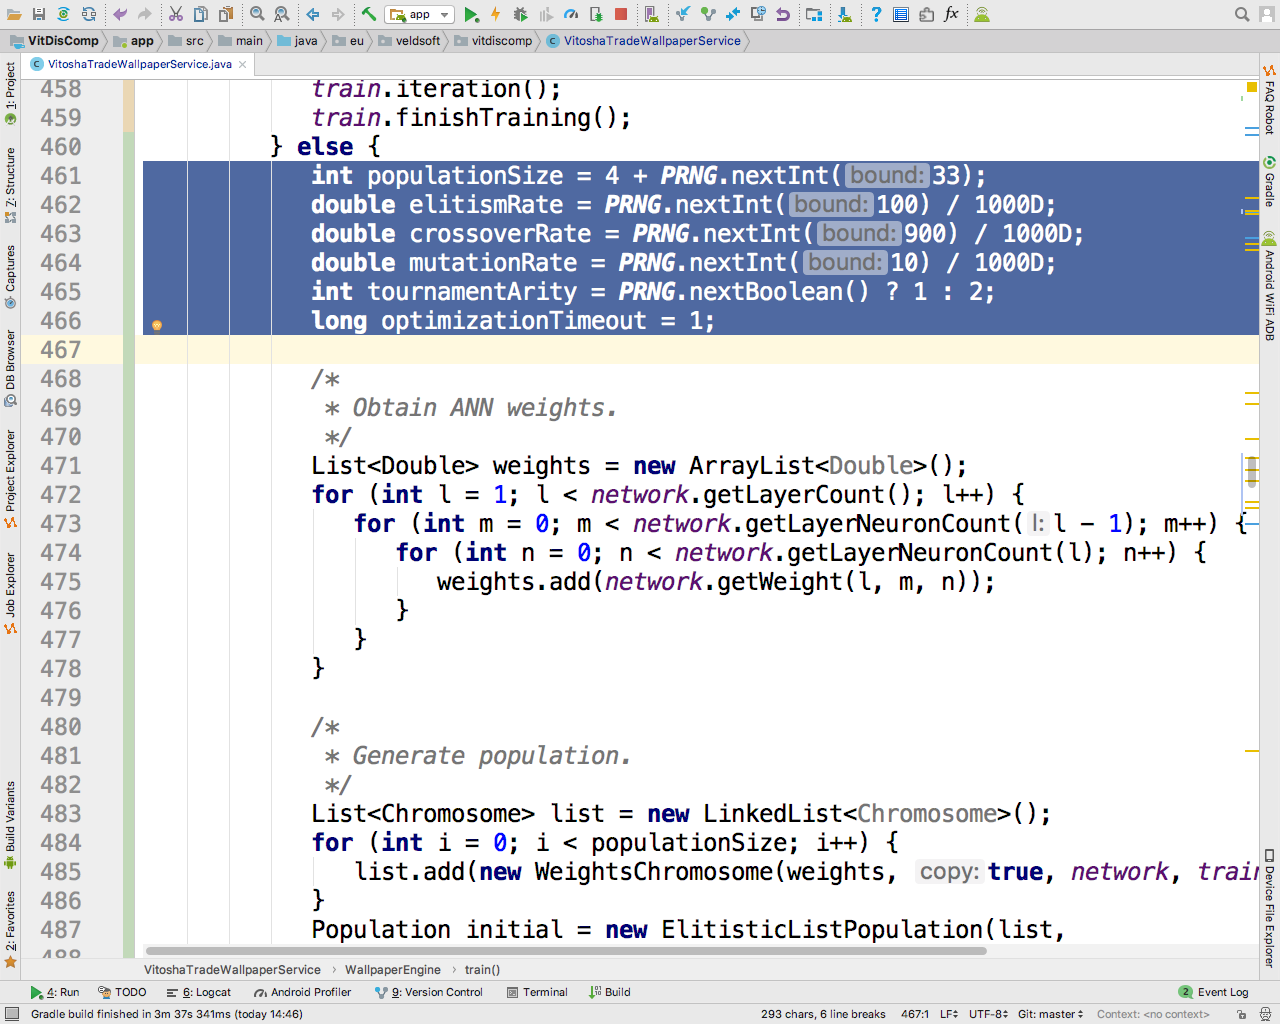
\includegraphics[height=0.45\pdfpageheight]{pic0179}
\caption{Genetic Algorithm Parameters}
\label{fig:pic0179}
\end{figure}
\FloatBarrier

The genetic algorithm is tuned with a set of parameters (population size, percentage of elite in the population, crossover rate, mutation rate, number for the selection tournament, and the maximum number of seconds to perform optimization), which in this case are statically set. However, it is reasonable to be controlled by a configuration file or a settings screen (Fig. \ref{fig:pic0179}).

\begin{figure}[h]
\centering
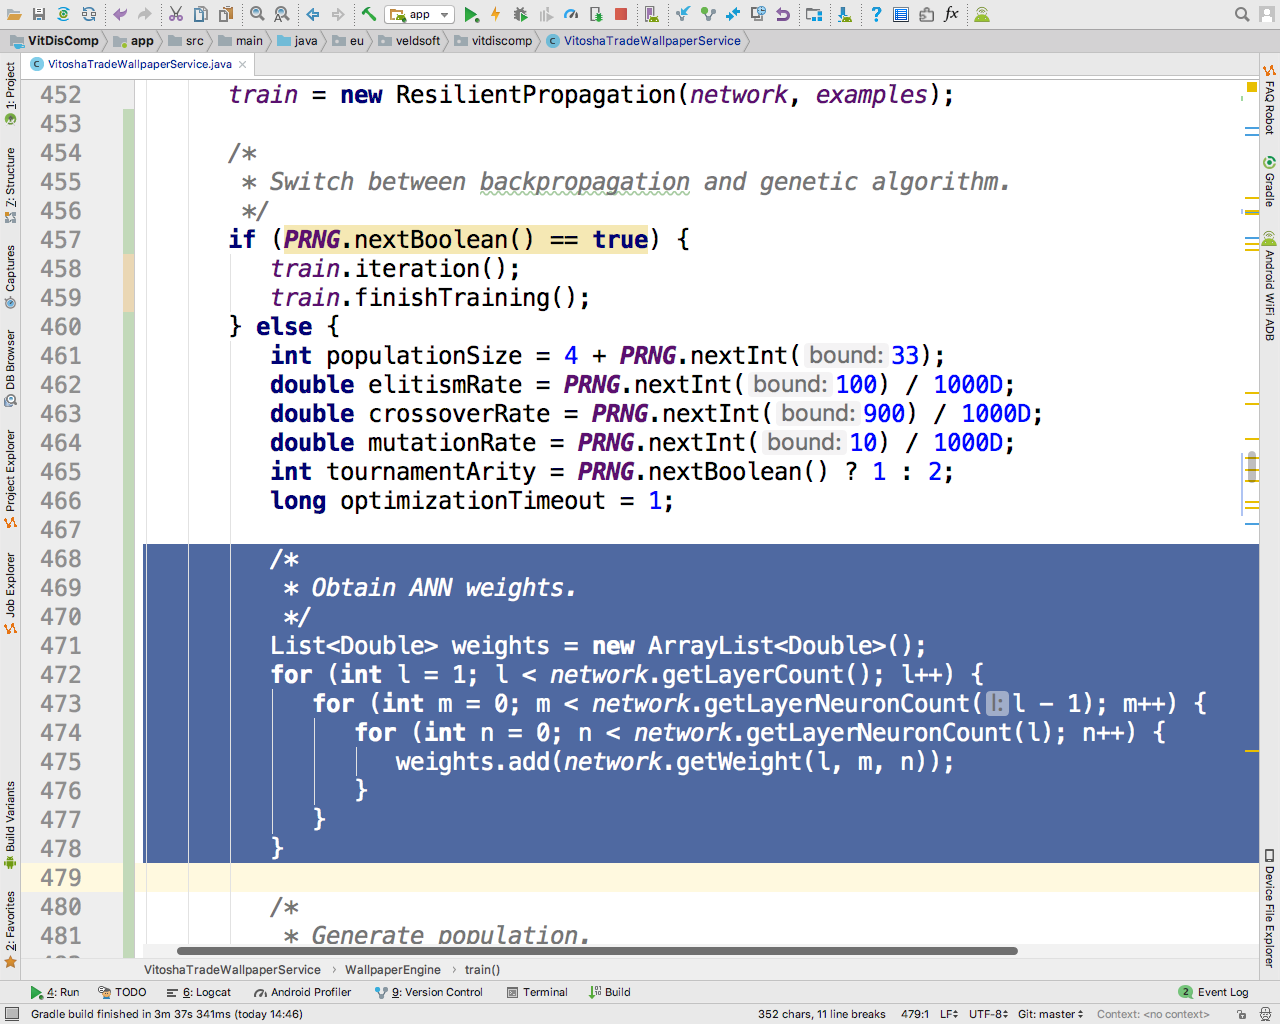
\includegraphics[height=0.45\pdfpageheight]{pic0180}
\caption{Retrieving the weights from the network}
\label{fig:pic0180}
\end{figure}
\FloatBarrier

The network weights are arranged in a vector of real values (Fig. \ref{fig:pic0180}).

\begin{figure}[h]
\centering
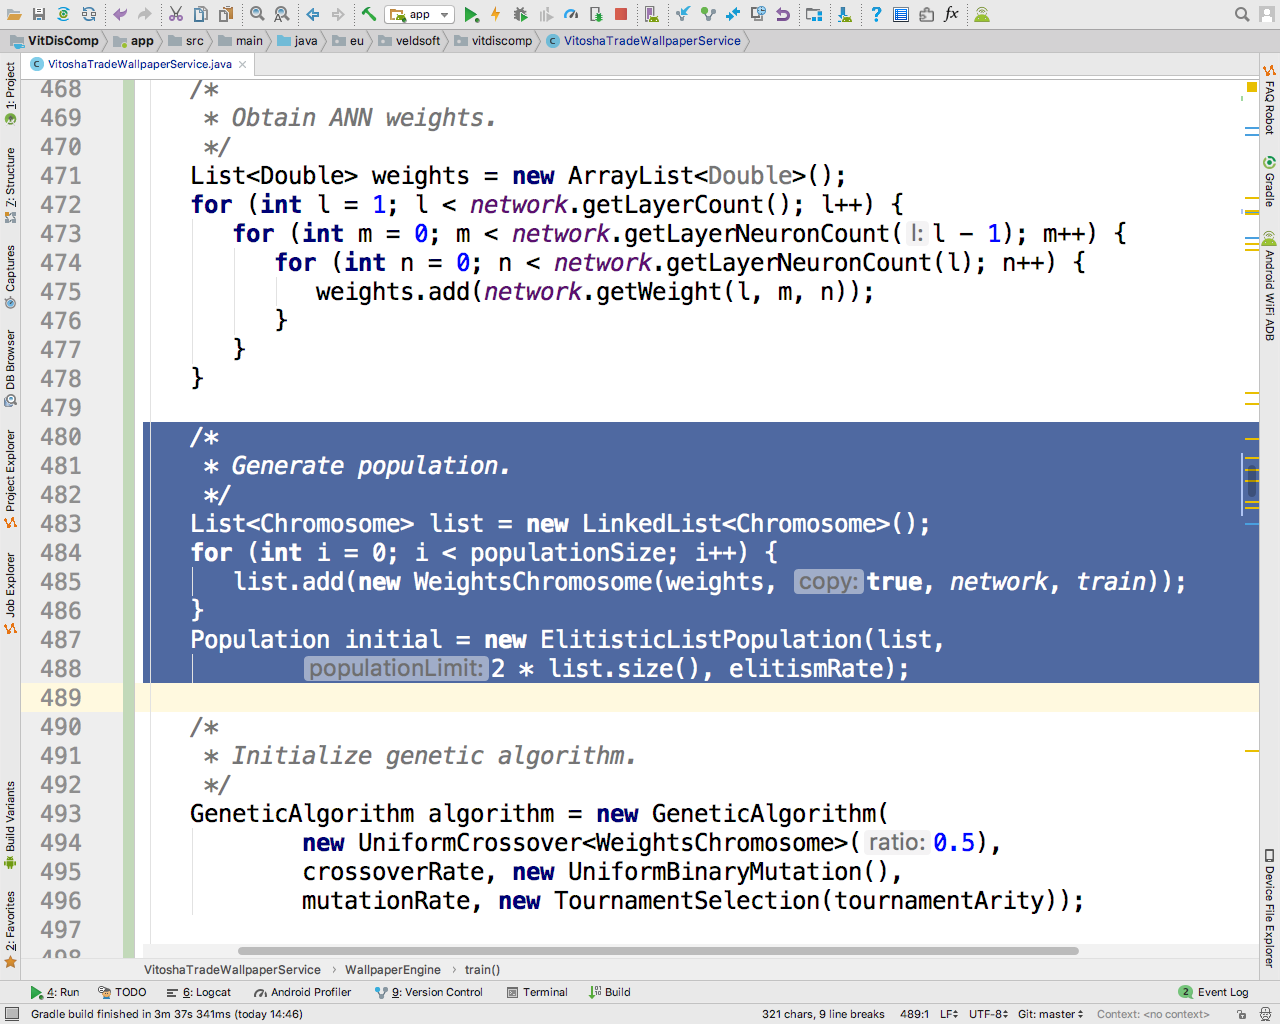
\includegraphics[height=0.45\pdfpageheight]{pic0181}
\caption{Initial population}
\label{fig:pic0181}
\end{figure}
\FloatBarrier

An initial population is formed from the extracted weights to start the optimization (Fig. \ref{fig:pic0181}).

\begin{figure}[h]
\centering
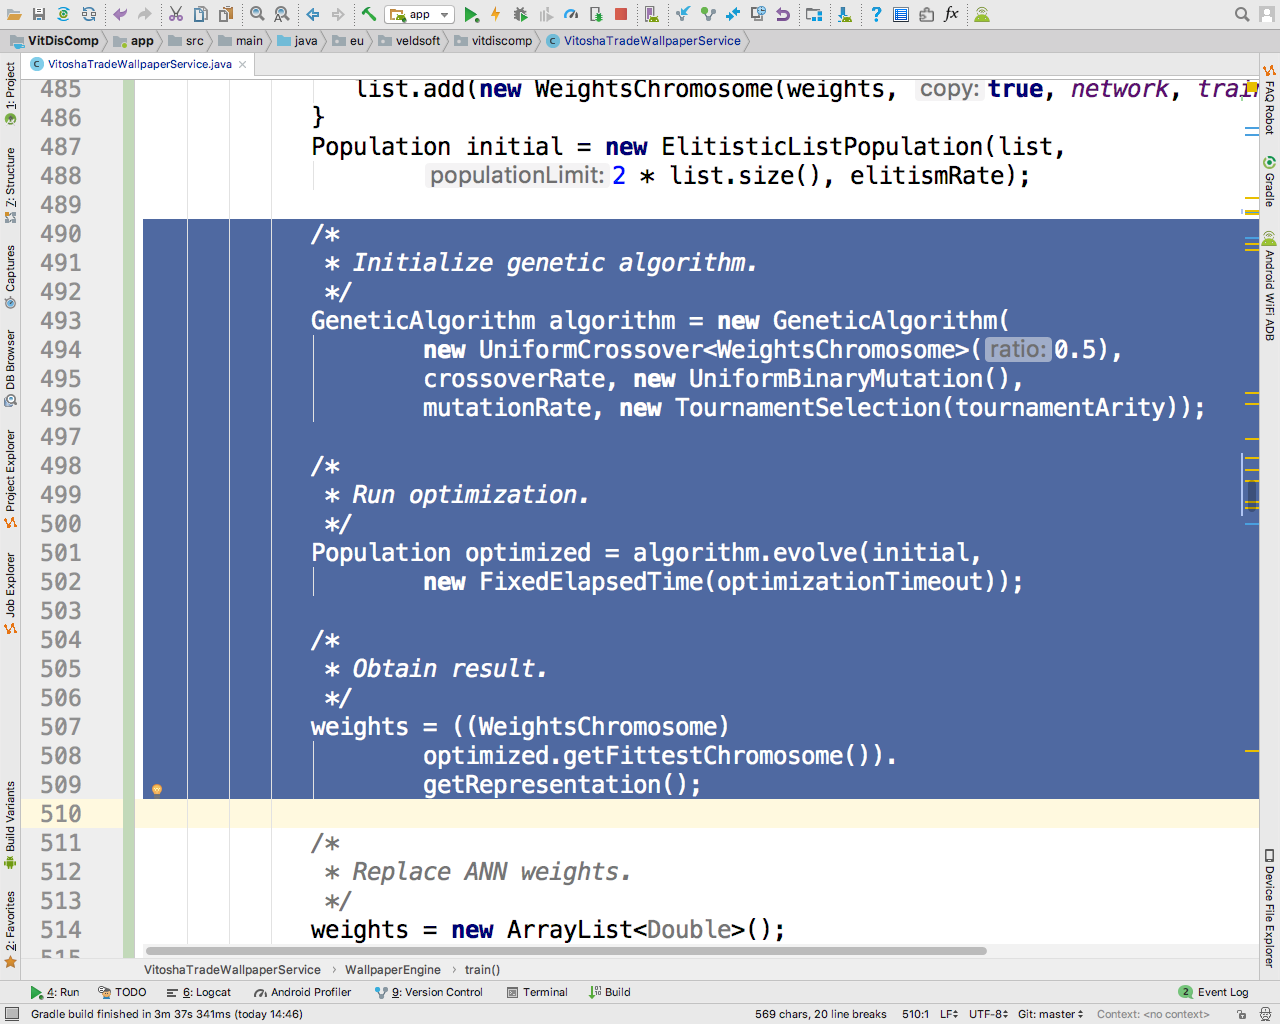
\includegraphics[height=0.45\pdfpageheight]{pic0182}
\caption{Genetic Algorithm Execution}
\label{fig:pic0182}
\end{figure}
\FloatBarrier

An implementation of the genetic algorithm follows (Fig. \ref{fig:pic0182}). A uniform random crossover is applied for crossover. For mutation, a uniform binary mutation is applied to all genes on the chromosome. The best individual from the optimized population is loaded back into the network (Fig. \ref{fig:pic0183}).

\begin{figure}[h]
\centering
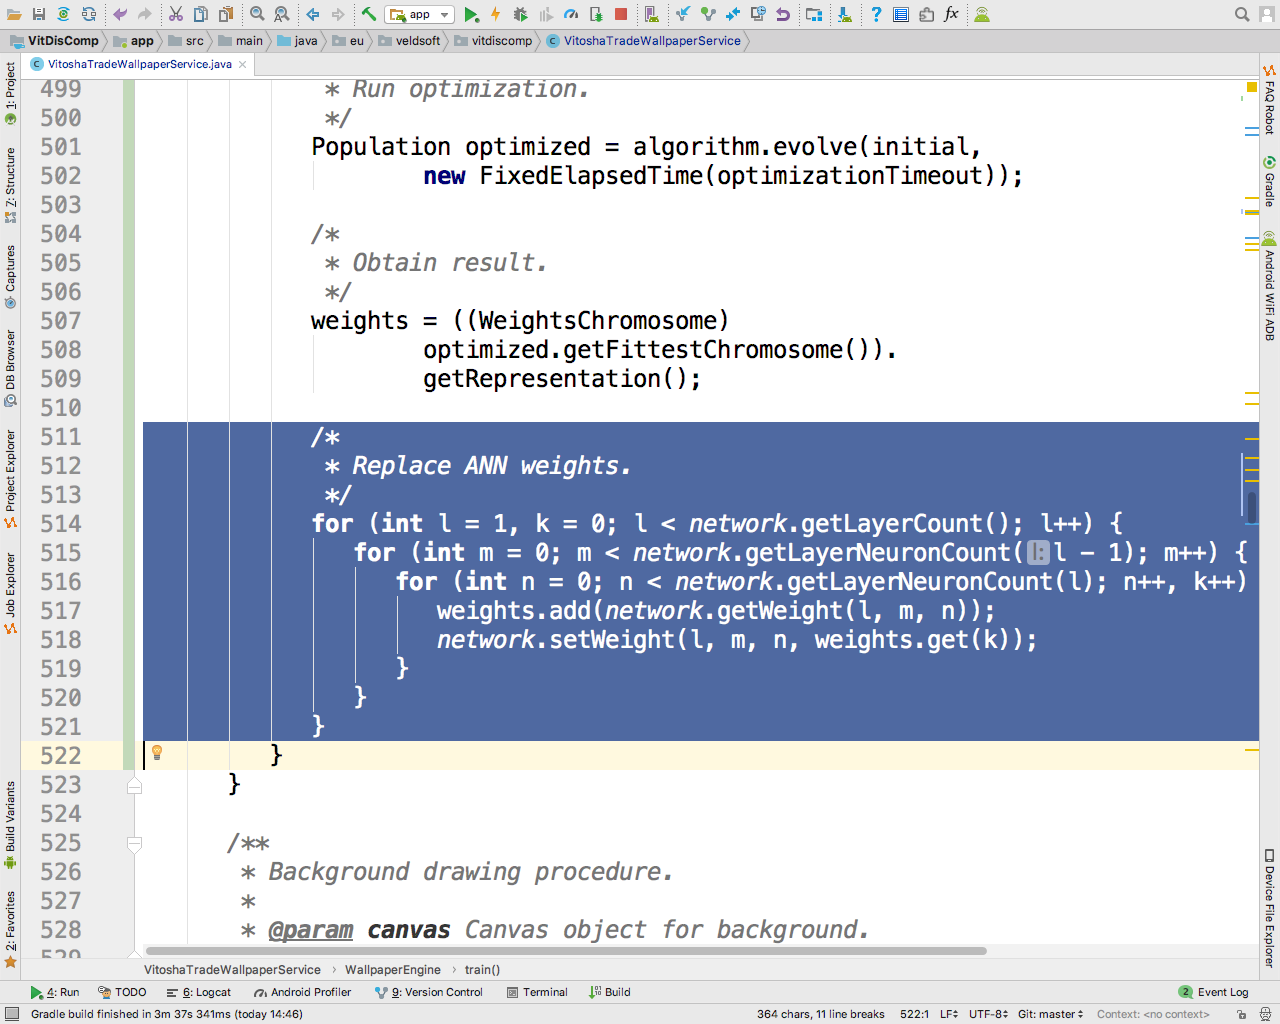
\includegraphics[height=0.45\pdfpageheight]{pic0183}
\caption{Update network weights}
\label{fig:pic0183}
\end{figure}
\FloatBarrier

\subsection{Chromosome Coding}

Since the network weights are a set of real numbers, they can ideally be represented in a chromosome containing a list of values (Fig. \ref{fig:pic0184}). Since the fitness estimation requires the weights to be loaded into the network and the straight-pass backpropagation training run over the network, the chromosome contains references to the network object and the training object.

\begin{figure}[h]
\centering
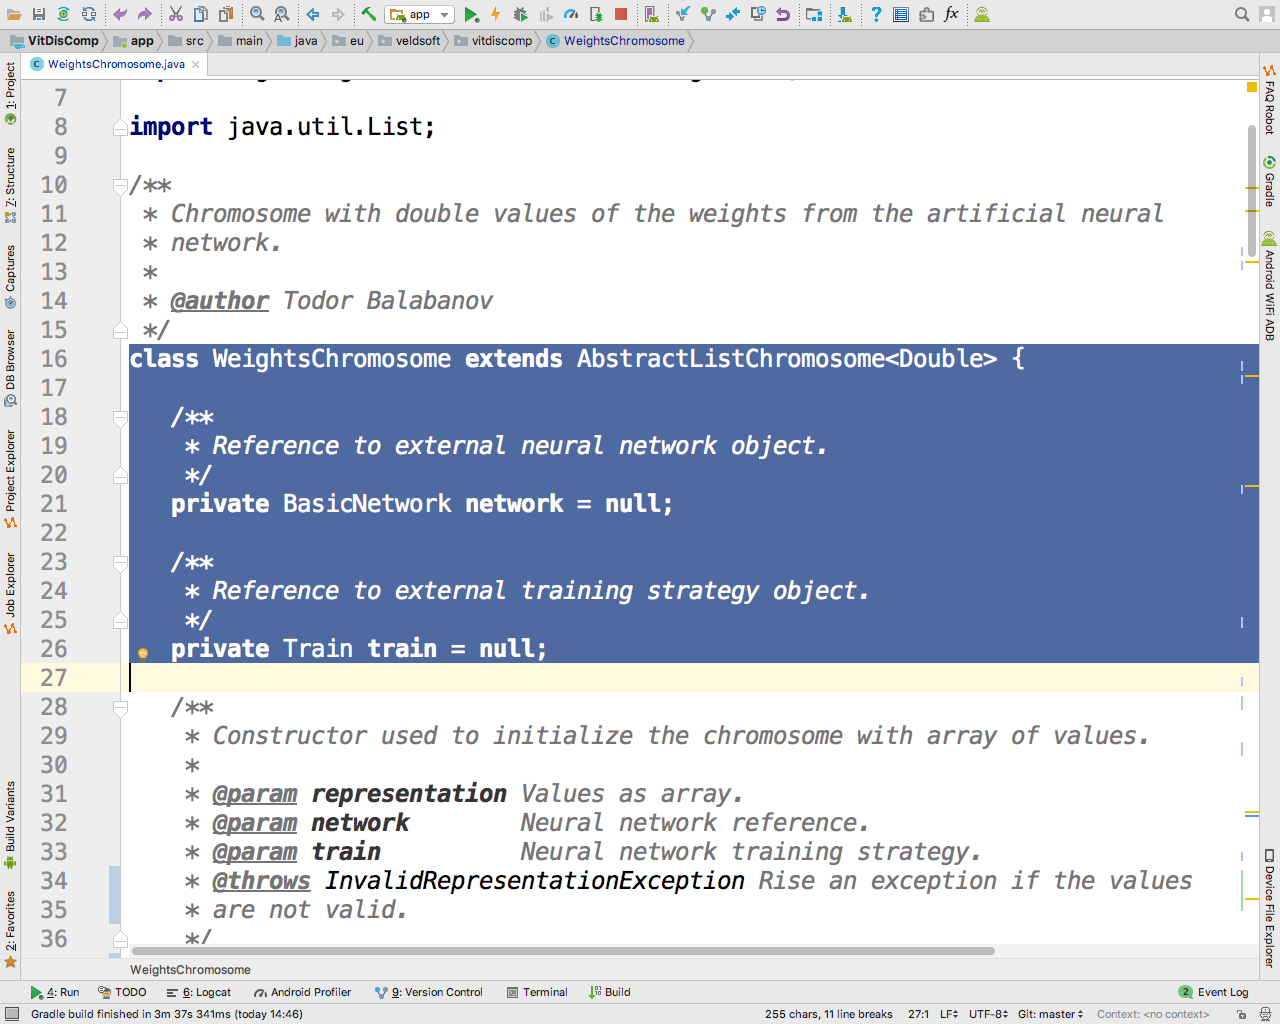
\includegraphics[height=0.45\pdfpageheight]{pic0184}
\caption{Encoding the weights in the chromosomes}
\label{fig:pic0184}
\end{figure}
\FloatBarrier

For flexibility in creating the chromosome objects, the three inherited constructors have been redefined (Fig. \ref{fig:pic0185}, Fig. \ref{fig:pic0186}, Fig. \ref{fig:pic0187}).

\begin{figure}[h]
\centering
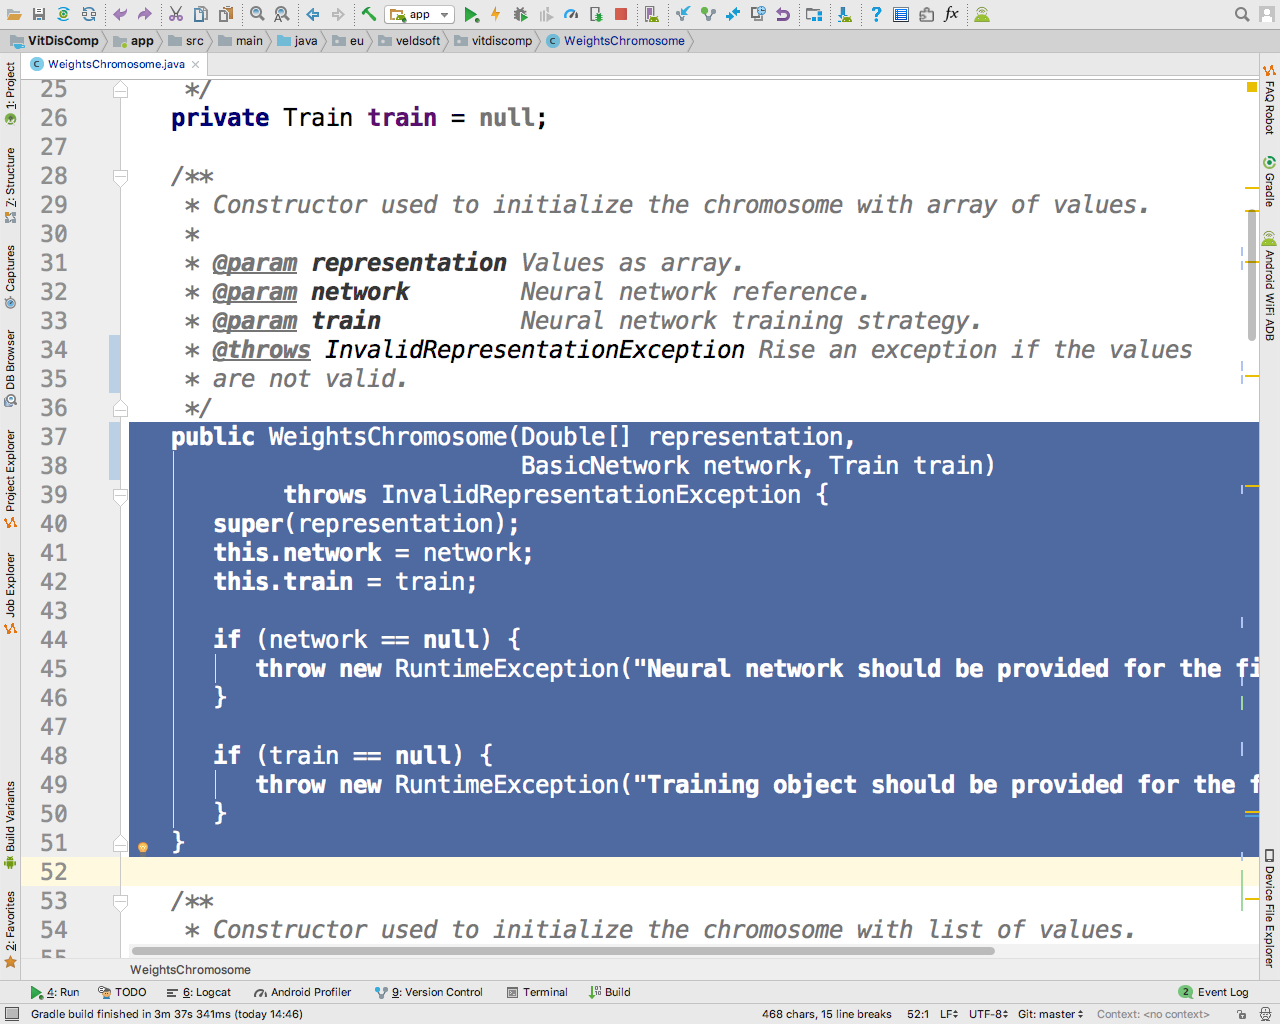
\includegraphics[height=0.45\pdfpageheight]{pic0185}
\caption{Construction by given array}
\label{fig:pic0185}
\end{figure}
\FloatBarrier

\begin{figure}[h]
\centering
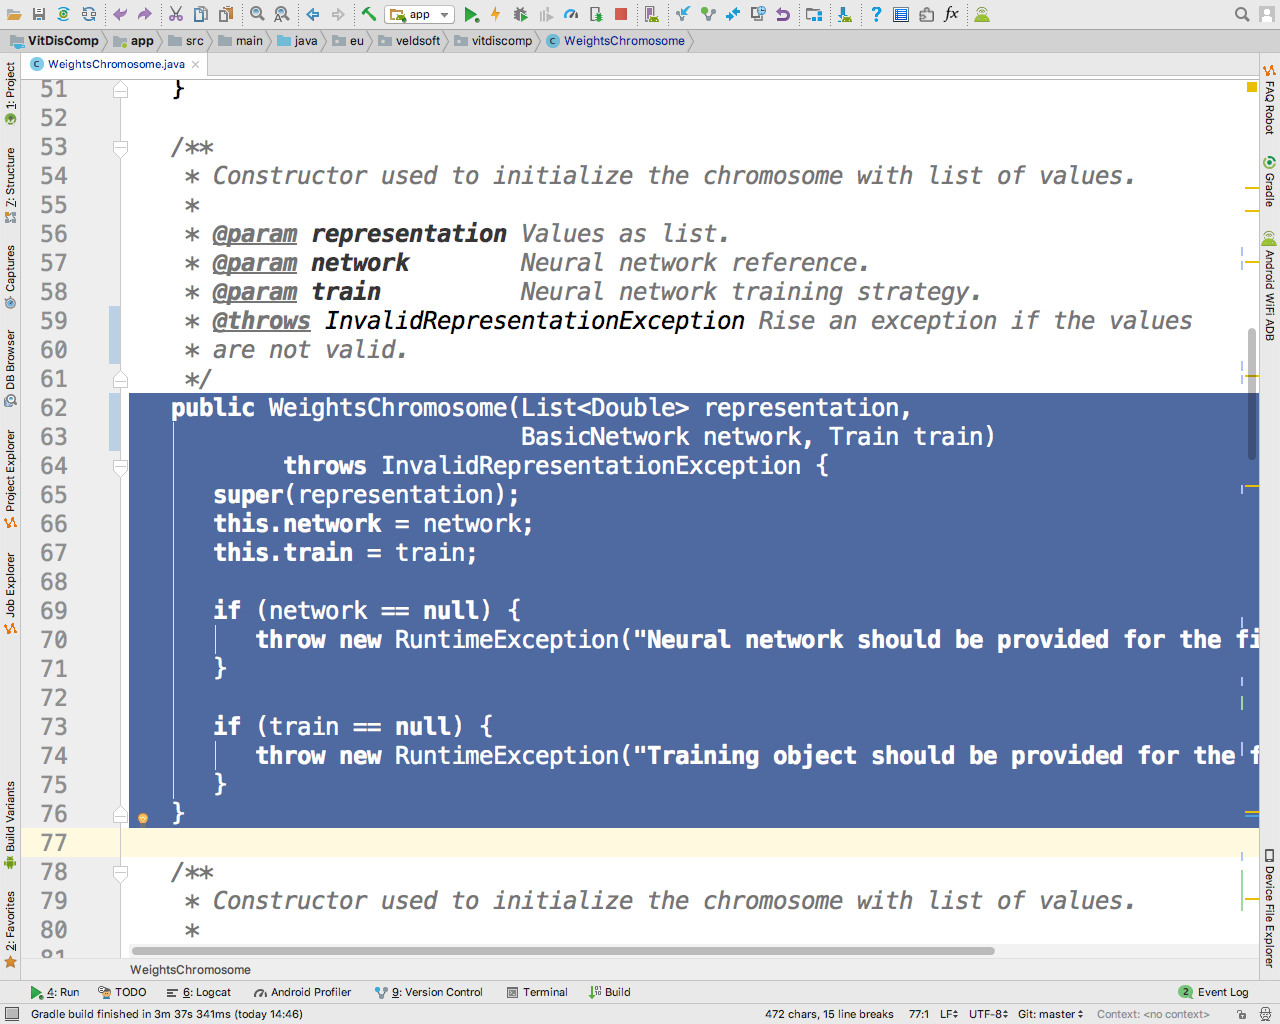
\includegraphics[height=0.45\pdfpageheight]{pic0186}
\caption{Build by set list}
\label{fig:pic0186}
\end{figure}
\FloatBarrier

\begin{figure}[h]
\centering
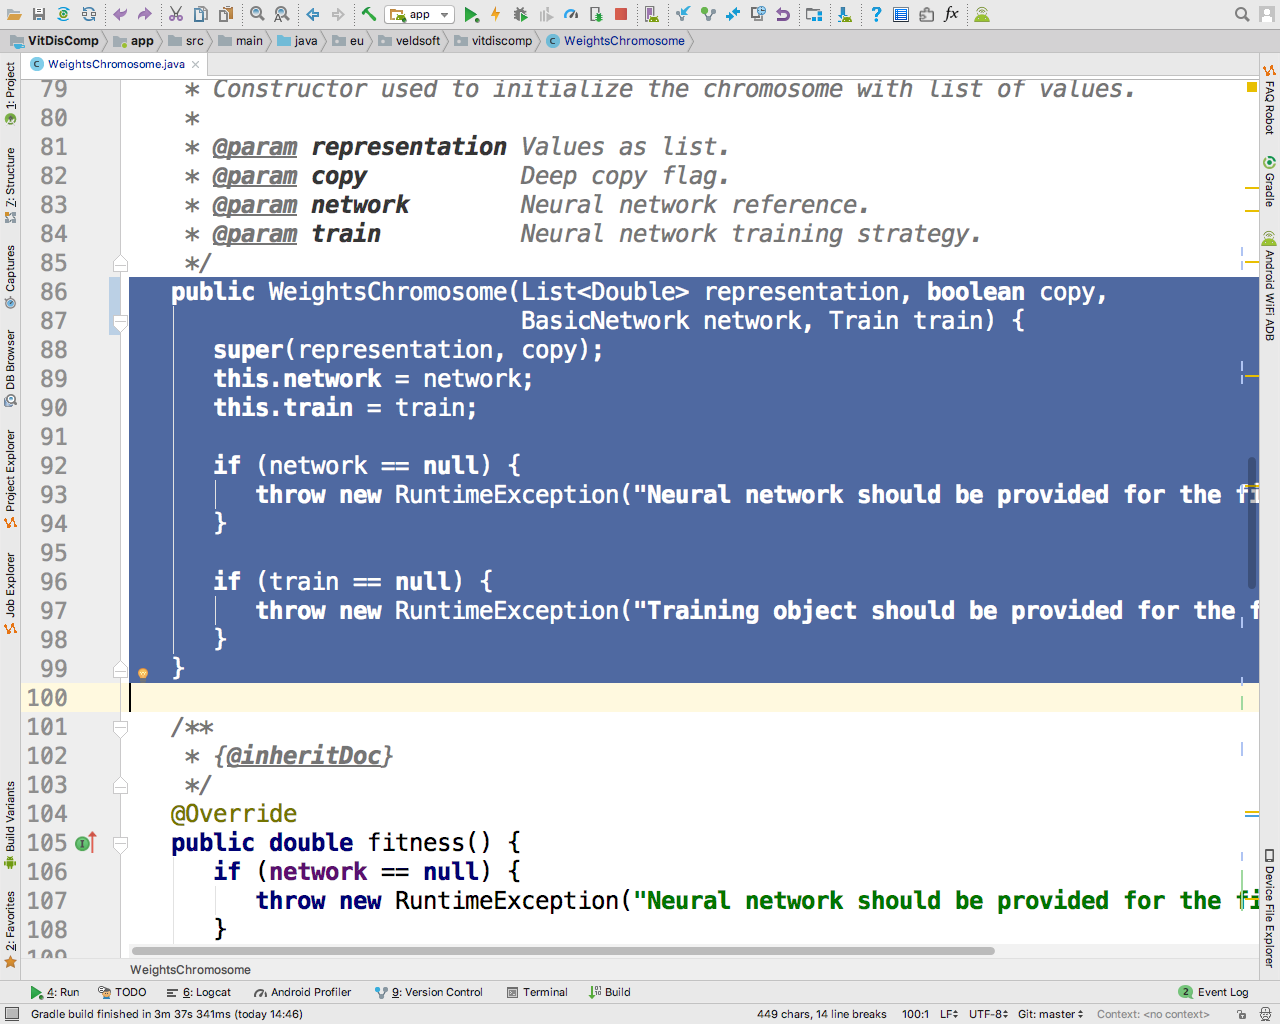
\includegraphics[height=0.45\pdfpageheight]{pic0187}
\caption{Deep-copyable set-list construction}
\label{fig:pic0187}
\end{figure}
\FloatBarrier

Fitness estimation begins by loading the fractional values as weights into the artificial neural network (Fig. \ref{fig:pic0188}).

\begin{figure}[h]
\centering
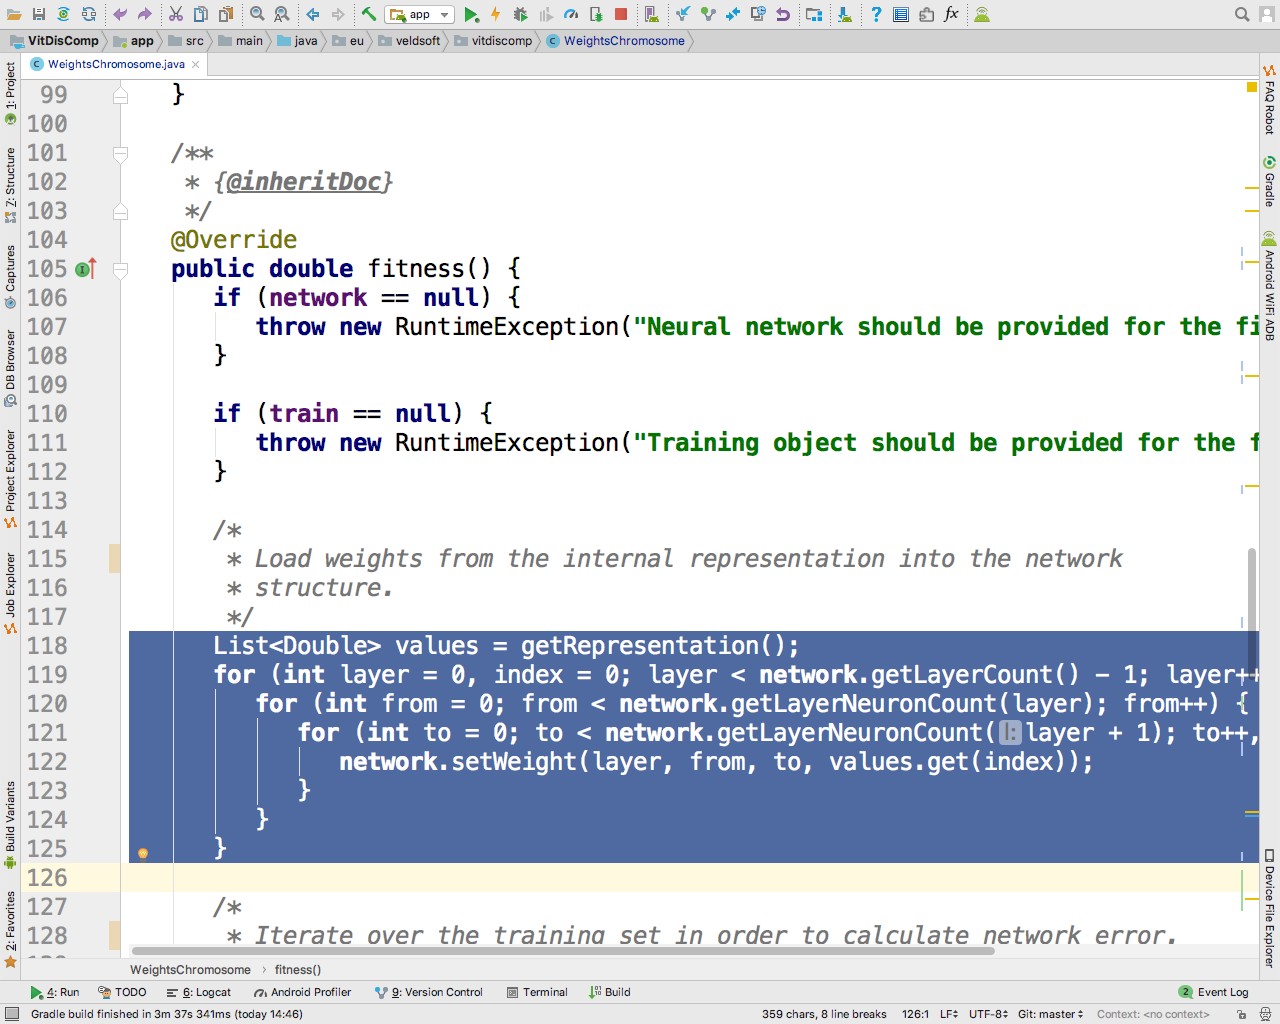
\includegraphics[height=0.45\pdfpageheight]{pic0188}
\caption{Loading the values as weights into the network}
\label{fig:pic0188}
\end{figure}
\FloatBarrier

The forward pass is performed, and the total error committed by the network is returned as a fitness value (Fig. \ref{fig:pic0189}).

\begin{figure}[h]
\centering
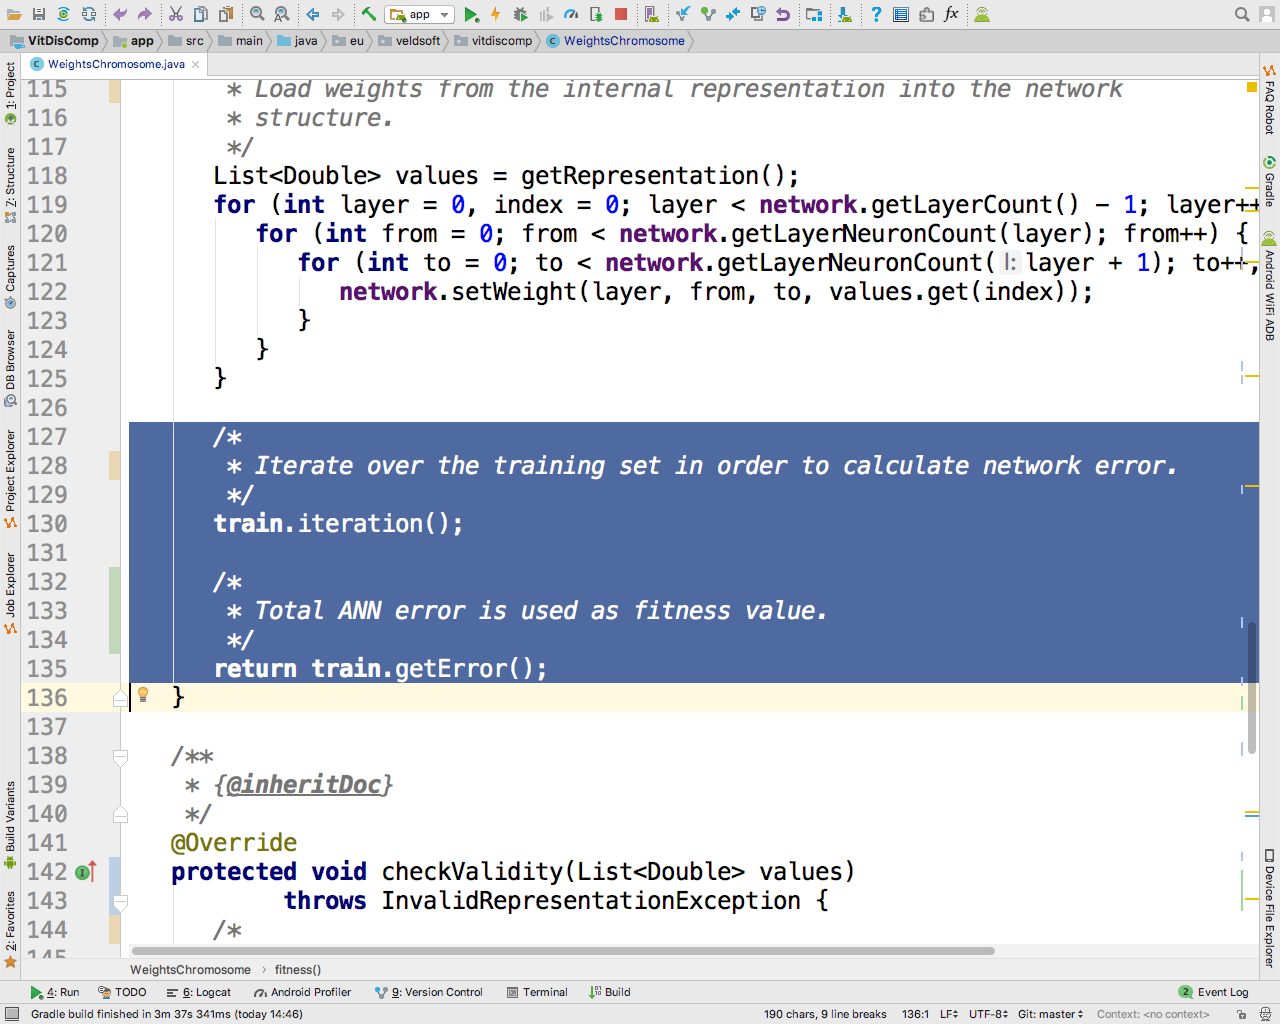
\includegraphics[height=0.45\pdfpageheight]{pic0189}
\caption{Executing the straight pass}
\label{fig:pic0189}
\end{figure}
\FloatBarrier

The validity of the chromosome depends only on having enough fractional numbers such that a value is assigned for each weight in the network (Fig \ref{fig:pic0190}).

\begin{figure}[h]
\centering
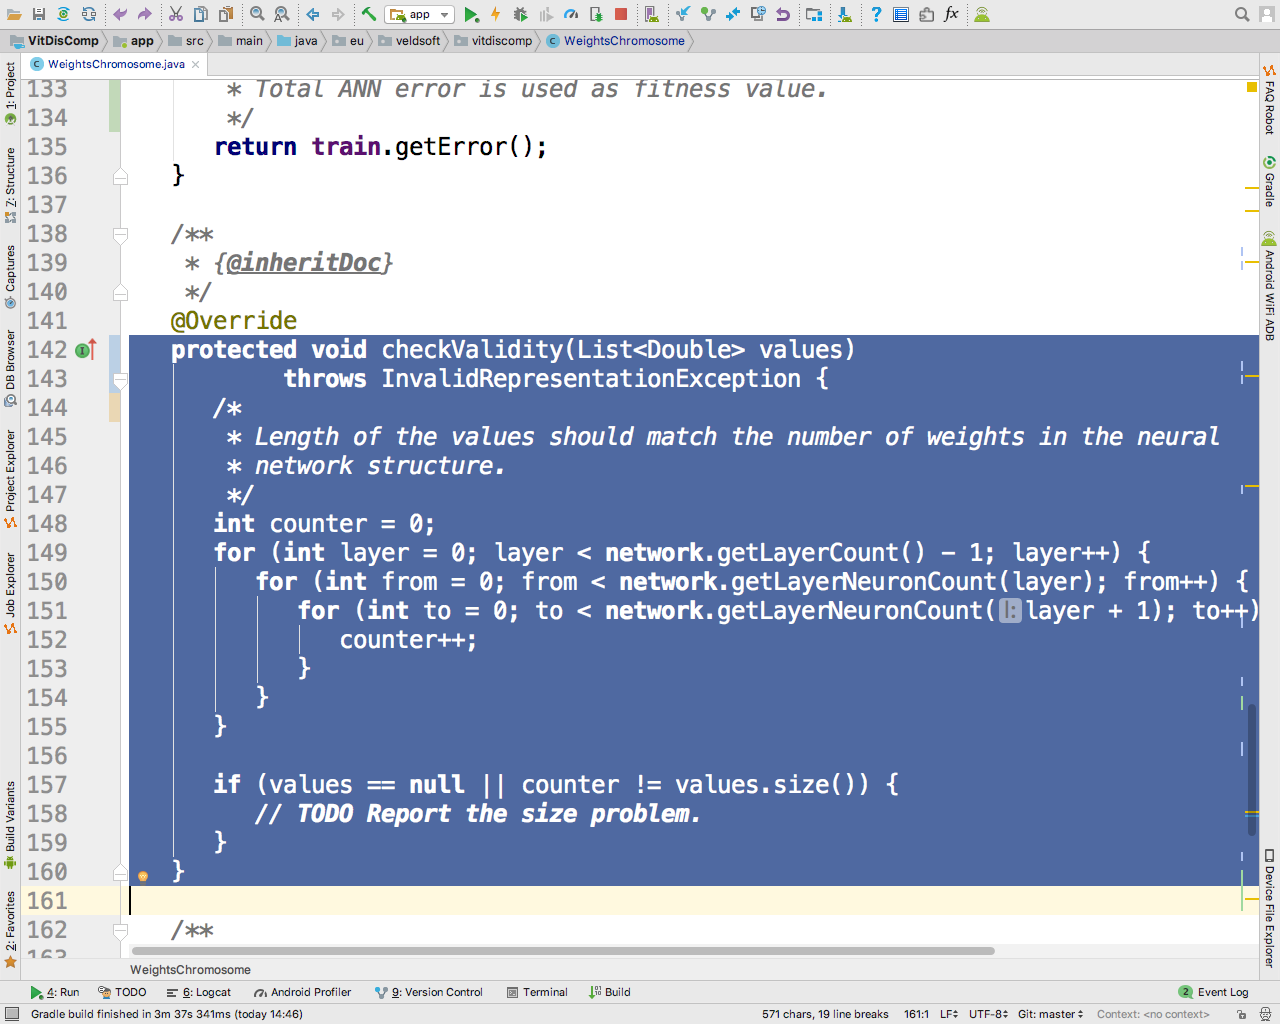
\includegraphics[height=0.45\pdfpageheight]{pic0190}
\caption{Chromosome validity condition}
\label{fig:pic0190}
\end{figure}
\FloatBarrier

Constructing a new chromosome of fixed length is done by calling one of the constructors and using a deep copy for the values (Fig. \ref{fig:pic0191}).

\begin{figure}[h]
\centering
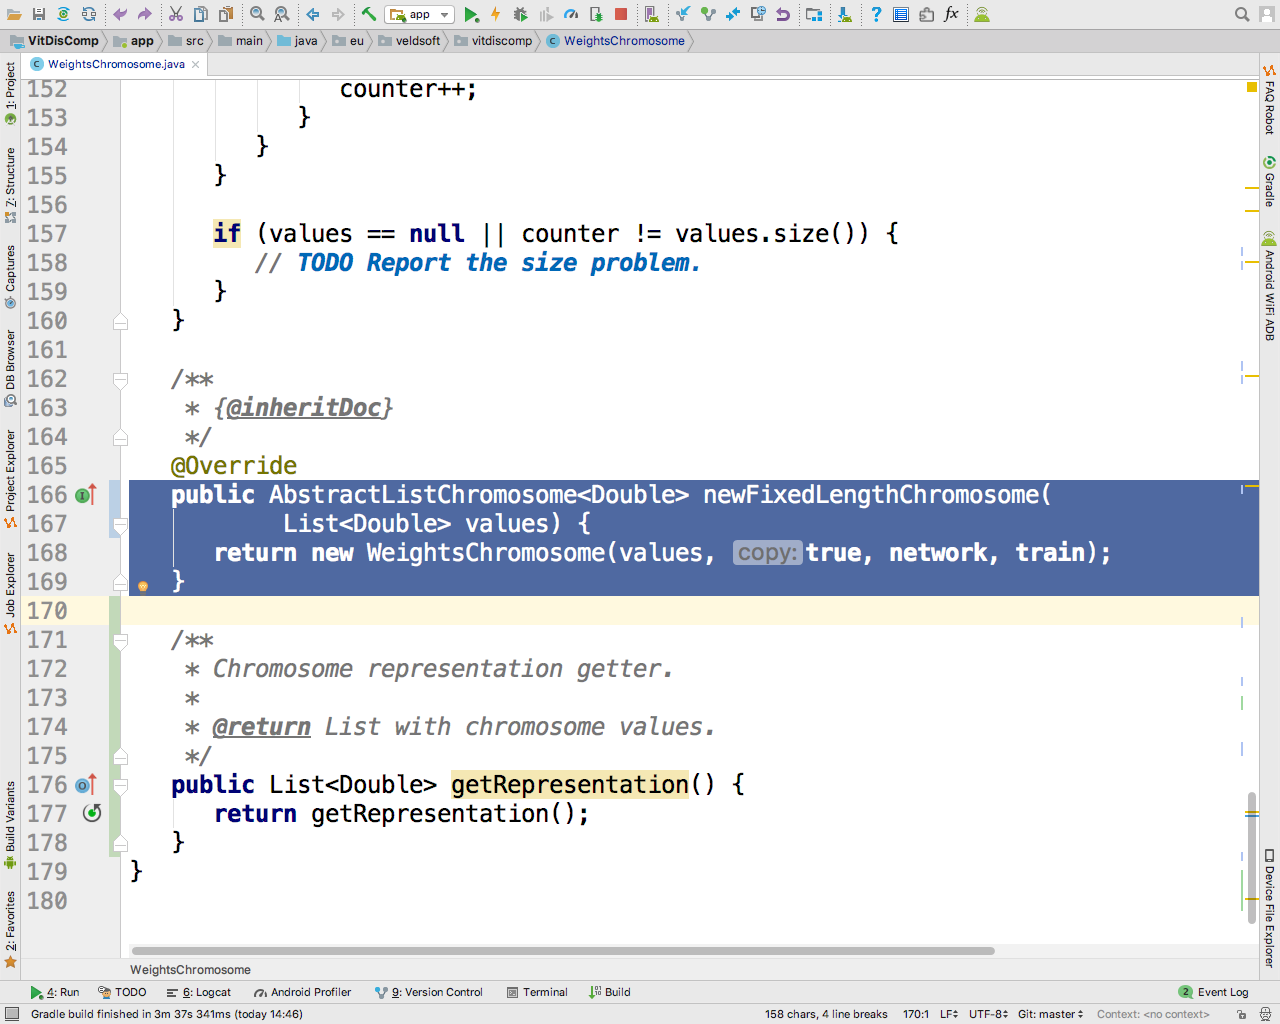
\includegraphics[height=0.45\pdfpageheight]{pic0191}
\caption{Construction of a new chromosome of fixed length}
\label{fig:pic0191}
\end{figure}
\FloatBarrier

A function was created for calculations outside the class to output the values (Fig. \ref{fig:pic0192}).

\begin{figure}[h]
\centering
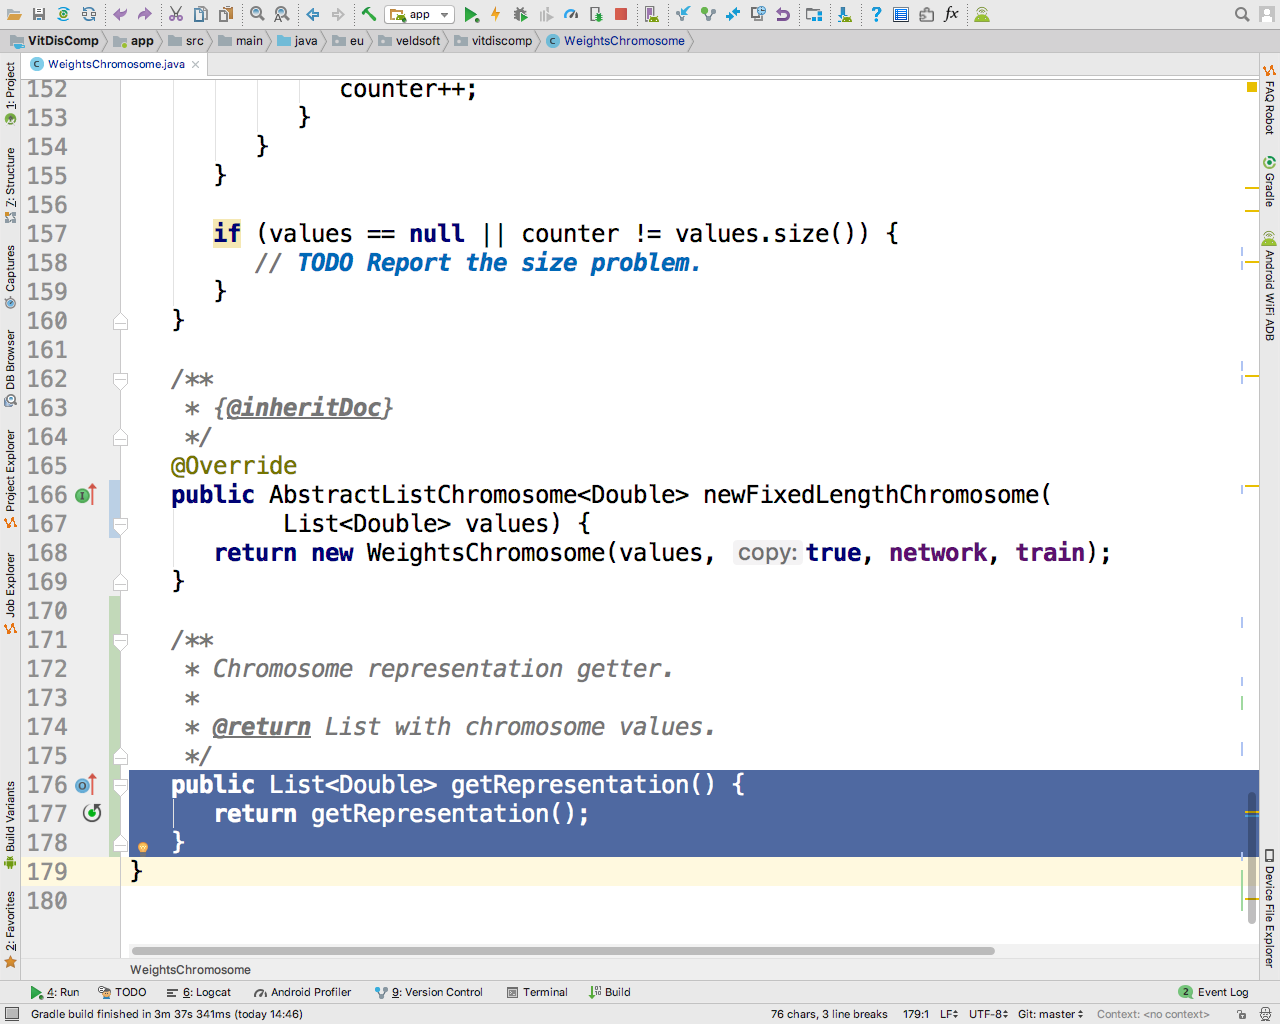
\includegraphics[height=0.45\pdfpageheight]{pic0192}
\caption{Function to output the values outside the chromosome}
\label{fig:pic0192}
\end{figure}
\FloatBarrier

\subsection{Random Uniform Mutation}

Since the Genetic Algorithms - Apache Commons library does not offer a suitable binary mutation for a vector of real numbers, a class implementing the mutation operation is proposed for development purposes (Fig. \ref{fig:pic0193}).

\begin{figure}[h]
\centering
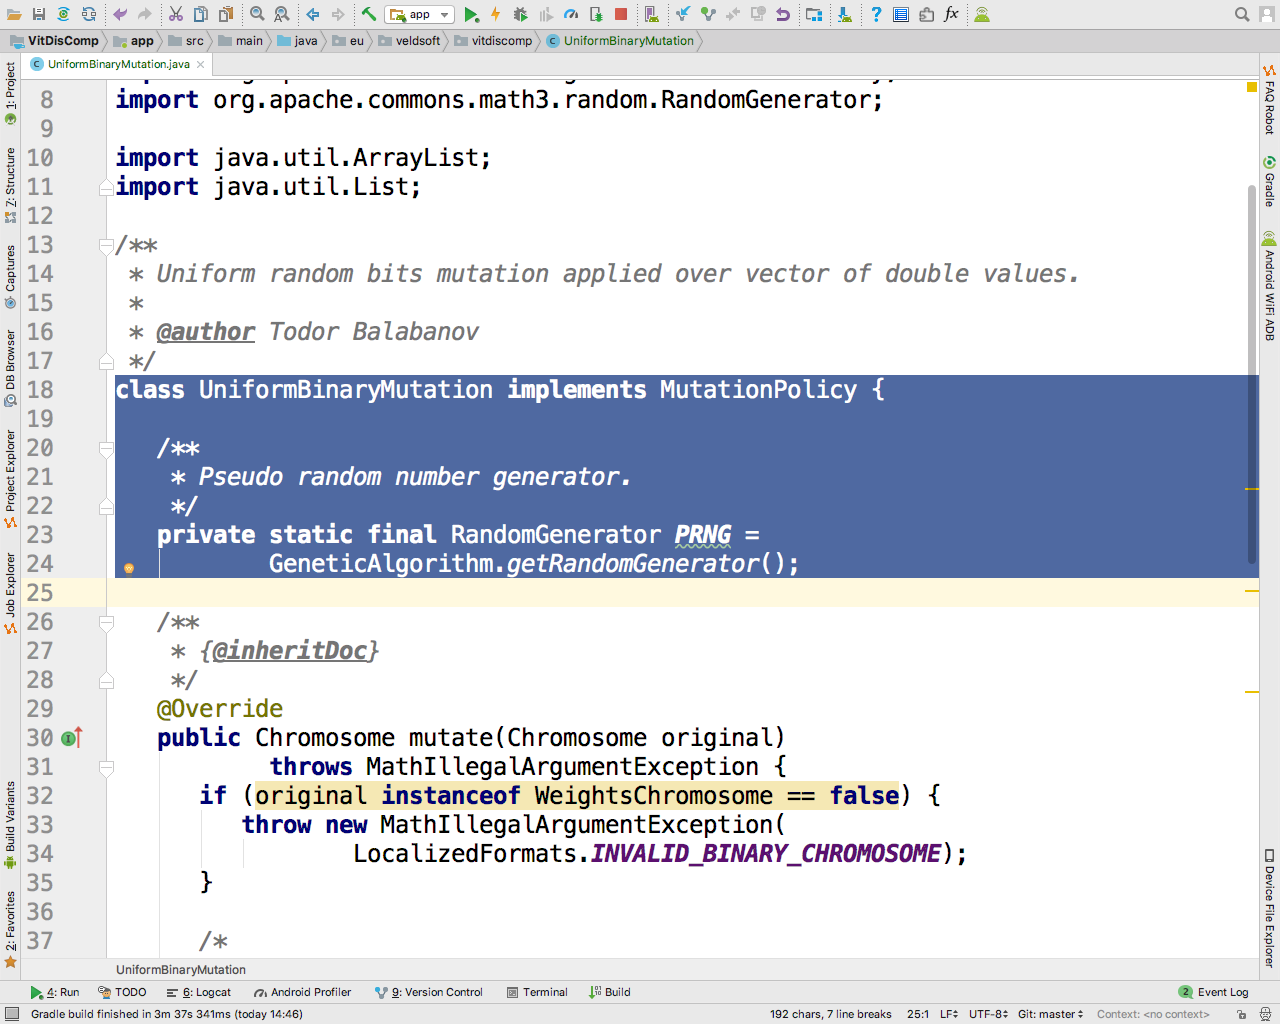
\includegraphics[height=0.45\pdfpageheight]{pic0193}
\caption{Class performing the mutation}
\label{fig:pic0193}
\end{figure}
\FloatBarrier

The proposed mutation operation is suitable to be applied only to the used coding in the chromosomes. For this reason, the mutation function performs the necessary validation on the input data (Fig. \ref{fig:pic0194}).

\begin{figure}[h]
\centering
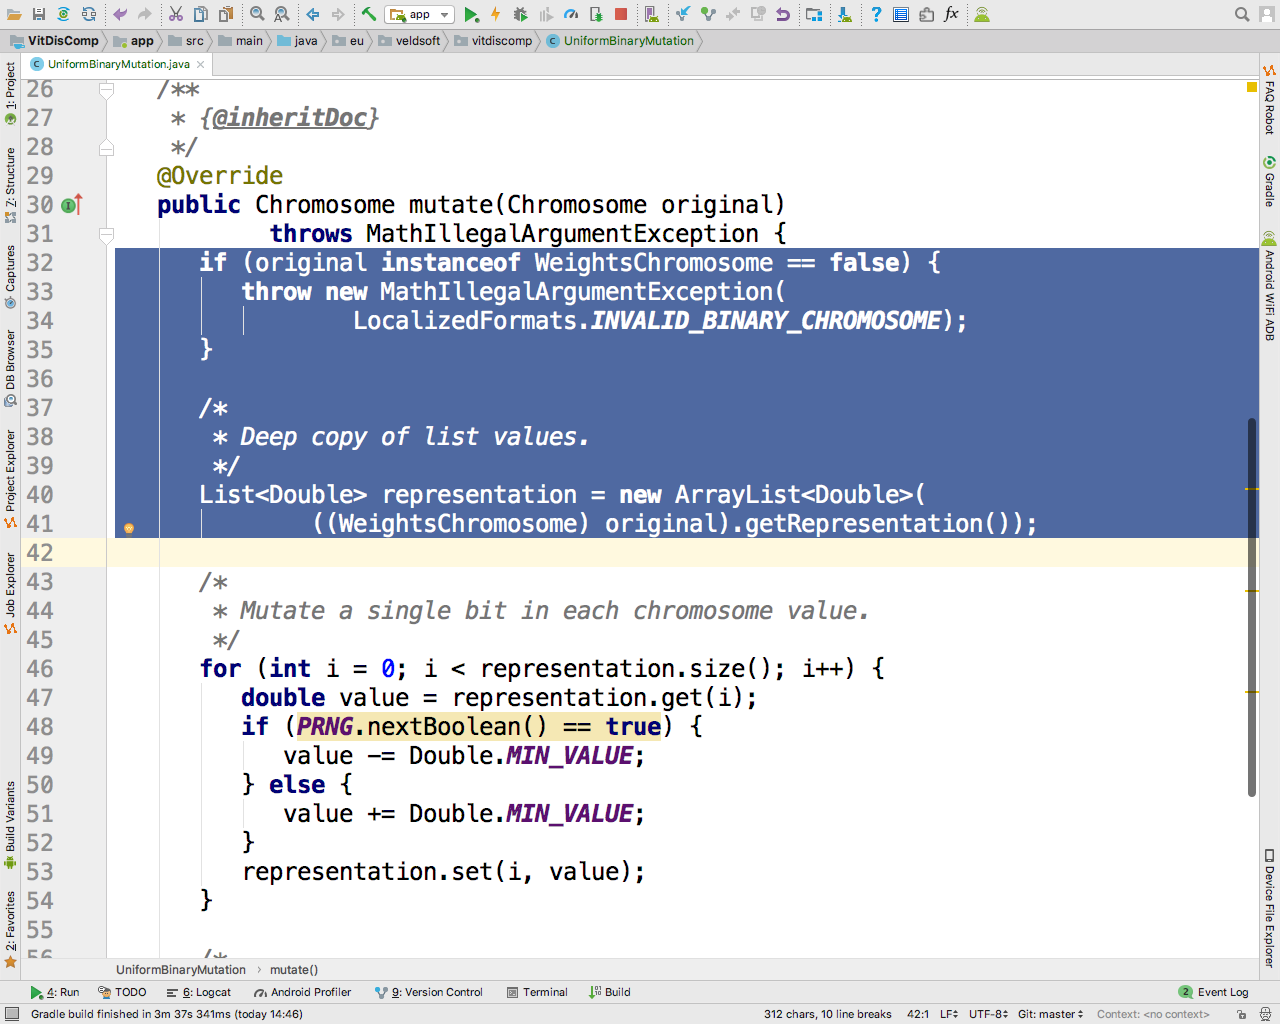
\includegraphics[height=0.45\pdfpageheight]{pic0194}
\caption{Input Control}
\label{fig:pic0194}
\end{figure}
\FloatBarrier

Unlike the classical mutation in genetic algorithms, a modification is made here, resembling the differential evolution method. A small fractional amount changes each gene in the chromosome (Fig. \ref{fig:pic0195}).

\begin{figure}[h]
\centering
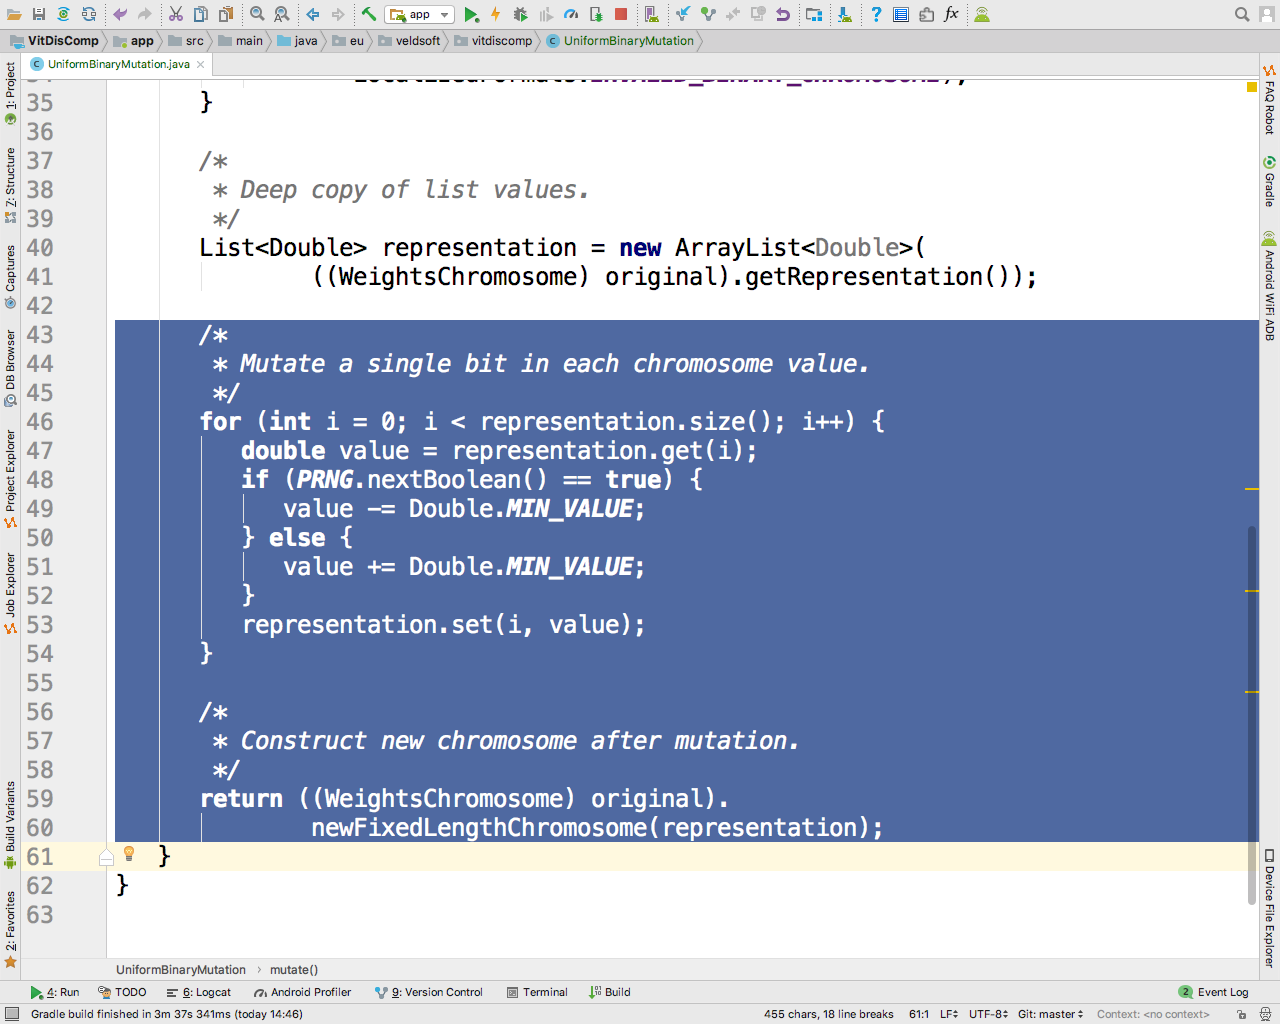
\includegraphics[height=0.45\pdfpageheight]{pic0195}
\caption{Random change of all values in the chromosome}
\label{fig:pic0195}
\end{figure}
\FloatBarrier

The mutation ends by creating and returning a mutated instance.
